\subsection{Detecting California Poppies}

We have also studied whether we can apply computer
vision analysis of Flickr photos to a problem of interest to
biologists: tracking the geo-temporal distribution of flowering
plants.  Plants and animals will respond as climates change over time,
and biologists would like fine-grained, continental scale information
about how flowering and migratory patterns are changing. Unlike
weather conditions, this data is very difficult to monitor from
satellites or aircraft, so biologists currently rely mostly on
traditional data collection techniques like longitudinal studies of
small plots of land by expert biologists. Analyzing Flickr images
could provide an alternative data source for these studies.

As a step in this direction, here we consider one particular
class of flower: the California Poppy. We chose this flower both because of its
distinct visual appearance (a bright orange) and because it is of
interest to biologists because it grows in a relatively
small area of the western U.S. and thus may be particularly
sensitive to changes in climate.

\subsubsection*{Dataset}

From our collection of about 100 million U.S. Flickr photos, we selected
all images tagged ``poppy'' (about  8100 images). Some
of these images are of  California Poppies but most are not, since
there are other species of poppies and amateur photographers often
confuse them with other flowers. We took a random sample of about 2000
images and asked biology  students to label them into one of
four categories: (1) close-up of a California Poppy; (2) multiple
California Poppies (e.g. in a photo of a field perhaps amongst other
flowers); (3) no California Poppy; and (4) special
cases like drawings of poppies.  We discarded images from category (4) and
sampled from the remaining dataset to have an equal proportion of the 
three classes. This gave 150 training images and 450 independent test images.
Figure~\ref{fig:poppies} shows a few sample images from our dataset.

\begin{figure}[t]
\begin{center}
{\small{
\begin{tabular}{c|c|c}
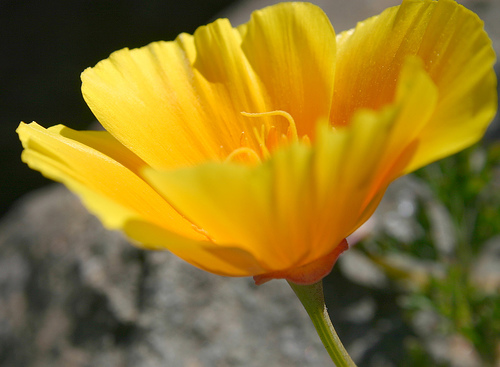
\includegraphics[width=0.13\textwidth]{figs/closeup1.jpg} &
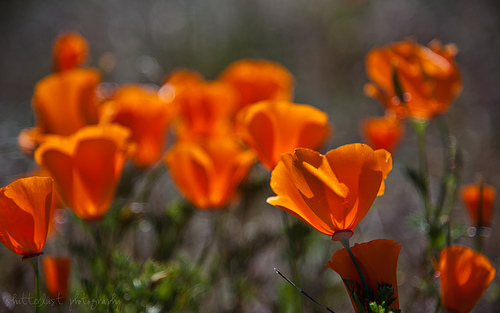
\includegraphics[width=0.13\textwidth]{figs/field1.jpg}& 
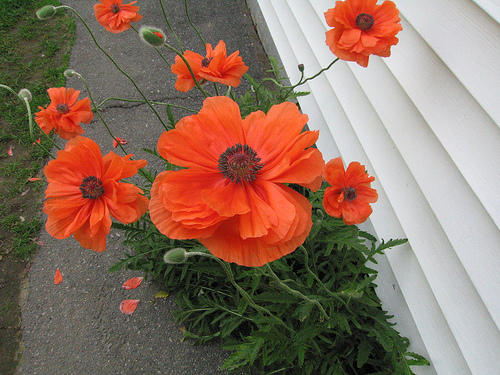
\includegraphics[width=0.13\textwidth]{figs/nopoppy1.jpg}
\\
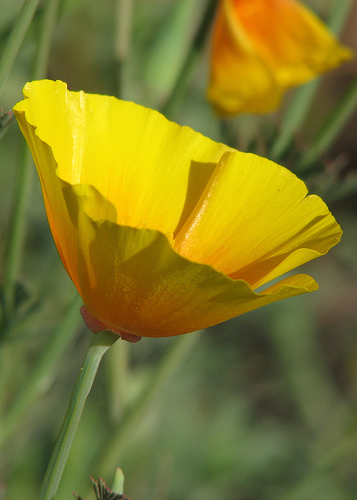
\includegraphics[height=0.8in]{figs/closeup2.jpg} &
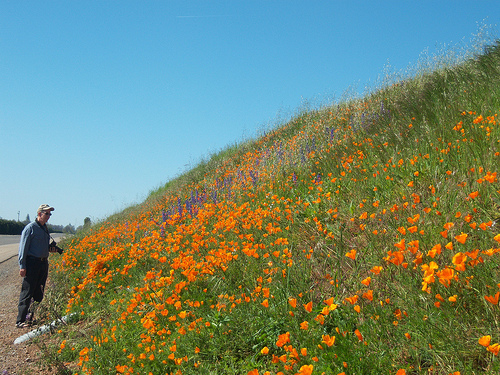
\includegraphics[width=0.13\textwidth]{figs/field2.jpg}& 
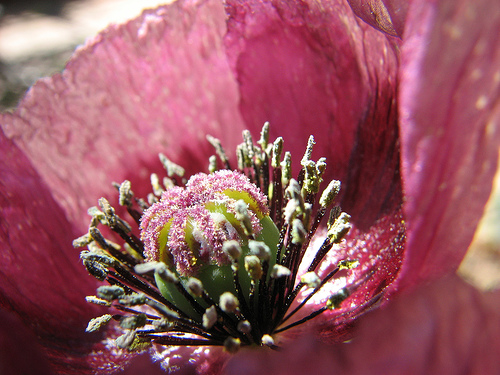
\includegraphics[width=0.13\textwidth]{figs/nopoppy2.jpg}
\\
%(a)&(b)&(c)\\
\end{tabular}
}}
\end{center}
\caption{
Some images from the three classes in our California Poppy dataset:
{\textit{(left):}} close-ups of true poppies;  
{\textit{(center):}} longer-range images of true poppies; and  {\textit{(right):}} images with no poppies.
}
\vspace{-12pt}
\label{fig:poppies}
\end{figure}

\subsubsection*{Classifying poppies}
We used the same features described above in Section~\ref{sec:snow}
for classifying snow images, including tiny images, color histograms,
color-aware local binary pattern with spatial pyramids, and GIST.  For
comparison, we also implemented techniques based on bag-of-words
vocabularies of color, texture, and shape features that have been
applied to flower recognition in past work~\cite{flower2006cvpr}. 
In particular:

%\begin{itemize}
\xhdr{Color vocabulary} 
We clustered the  HSV color values from
all images
 into a 200-word vocabulary,
and then represented each image as a histogram over these visual words.


%In order to reduce the effect of illumination variations, HSV value
%are used to describe the color feature. Each point of image will be
%represented as a 3-dimention vector. All the vectors of HSV value in
%training set are used to generate the K centers. For 150 training
%images, this input vector of function “kmeans” is as large as 1
%Gigabytes. On the server of tank.cs.indiana.edu, to avoid the problem
%of “out of memory”, the input is sampled 70\% from original
%images. And the best performance size of cluster K is 200 values
%currently.

%% \textbf{Getting visual words from training images}

%% Certain features (color, texture, etc.) are extracted from each
%% training image – this step will be discussed in detail later
%% respectively from each category. From the features in all training
%% images, generate K clustered centers (visual words) with k-mean
%% cluster. The size of the clustered center will be optimized for each
%% category based on the size of the features and of course,
%% performance. These clustered centers describe the most representative
%% instances of certain feature.

%% \textbf{Using frequency histogram to represent the images}

%% In terms of these clustered centers, frequency histograms are going to
%% be built for both training and testing images. These frequency
%% histograms would be representing the images for certain feature. From
%% the point of view of a certain feature, on the corresponding clustered
%% center, each testing image will be classified to the training image
%% with the smallest distance on frequency histograms.

%% \subsubsection{Building the visual vocabulary}

%% 	\textbf{Color Vocabulary}
	
\xhdr{Shape vocabulary} We use SIFT features to represent
  local image ``shape.'' We extracted SIFT features densely (on $25
  \times 25$ pixel regions,  at strides of 20 pixels), and
  again built a vocabulary using $k$-means clustering with $k=200$.

%% Scale invariant descriptor SIFT is used to describe shape feature of
%% poppy images. In my implementation, I used the vlfeat toolbox for
%% matlab [2]. This toolbox implements a number of visual algorithms. The
%% dense SIFT is extended from SIFT and was implemented one of the
%% original author of this algorithm [3]. It is applied on each 25*25
%% windows in each pre-smoothed image with 20 steps (pixels) away from
%% each other. Since SIFT is very computation intensive, the dense sift
%% reduce the complexity while avoid too sensitive descriptor.  Since
%% there are only 1000 to 2000 key points are selected in each image,
%% although it takes 128-dimensional vector to describe a key point, it
%% still won’t take too much space. So the input vector of kmean cluster
%% will keep the function within space capacity of the server. The best
%% performance K is now 200.

\xhdr{Texture vocabulary} We used MR8
  features~\cite{varma2002classifying} to capture local texture
  information.  MR8 applies a filter bank of 8 filters (4 Gaussians and 4 Laplacians of Gaussians) at different scales and orientations,
and then characterizes local texture in terms of the maximal filter responses. We again cluster these into a vocabulary with size 200.
%
%means the maximum response of 8 filters in
 % different scales. They are 4 in Gaussian filter and 4 in Laplacian
 % Gaussian of one circle and 3 in ecliptic in different shape and each
 % in 6 scales. \pleasenote{Jingya: They are 4 in Gaussian filter and 4 in Laplacian
 % filter. In Gaussian filter, there is one symmetric filter in circle, and 3 ecliptic filters in different scales, each scale gives the maximum respond at 6 orientations.}
 %In figure 1, the 14 different filters in MR4 are showed
 % in images. The maximum response of the 8 filters of each point will
 % be the texture feature descriptor. Clustered centers are generated
 % from 8-dimensional vectors of all the points in training image
 % set. This vector is large too. So 50\% percent of the points in
 % training image set are sampled from the training images. And the
 % best performance now is in K=200. \pleasenote{djc: Jingya, I don't
 %   completely understand this. There are 8 filters -- are these the 4
 %%   gaussian and 4 laplacian? Then for each of those there are 6 times
 %   3 = 18 variations? So then we choose the maximum response amongst
 %   these 18 for each of the 8 filter types. Is that right?  --------------------- There are 8 filters. They are the 4
 %   gaussian and 4 laplacian. There is 1 symmetric filter in guassian and 1 in laplacian. That gives 2. 
%The other 6 comes from 3 ecliptic filters with different scales in gaussian and laplacian respectively. 
%Each scale includes 6 orientations and only the maximum response will be chosen.
%There are 38 variations: 2 circular + 2*3(scales)*6(orientations) ecliptic, but every 6 orientations give only one maximum response.}

%\end{itemize}

We also define a combined feature which incorporates all three of the
above features. This feature computes the  histogram for
each of the three filters, and then concatenates these together after
normalizing  each vector.


%Combined Vocabulary is developed to improve the chance to get correct
%classification. All the histograms are normalized by the norm of the
%vector before the combining. The reason is easy to
%understand. Different feature gives different number of descriptors in
%each image. Hence, the actual values in histogram are different in
%scales. Without normalization, the texture vocabulary with the largest
%point in histogram will dominate the combined descriptor, therefore,
%the classification result.  The normalized histogram is%
%
%$\frac{v_{1}}{||v||},\frac{v_{2}}{||v||}...\frac{v_{n}}{||v||}$
%
%
%we used a weighted vector to combine normalized histograms. The weight
%is optimized and is mostly depend on the performance of each
%vocabulary. The best performance now is (0.4, 1, 1) as for color,
%shape and texture.

% The up to now best performance of combined vocabulary on 50 images in each training category is 65\%.


\subsubsection*{Results}

Table~\ref{tab:global_features} shows the performance of the different 
features on the problem of classifying close-up California Poppy photos
versus photos of fields and non-poppies. We observe that the vocabulary-based
features work significantly better in combination than separately, yielding
a combined accuracy of 65.0\% versus the 33.3\% baseline. The LBP, Gist, and LBP features perform better, with the best performance achieved by the combination of features (72.1\%).
Figure~\ref{fig:PR_ROC_poppy}  shows ROC and Precision-Recall curves.



\begin{table}
{\footnotesize{
\begin{center}
\begin{tabular}{|l|c|}
\hline 
Feature  & Accuracy\tabularnewline
\hline 
\hline 
Random Baseline  & 33.3\%\tabularnewline
\hline 
\hline
Shape Vocabulary & 45.0\% \tabularnewline
\hline 
Texture Vocabulary & 48.6\%\tabularnewline
\hline 
Color Vocabulary & 53.6\%\tabularnewline
\hline 
Combination of color, shape and texture  & \textbf{65.0\%}\tabularnewline
\hline
\hline
Tiny Image & 58.8\%\tabularnewline
\hline 
RGB histogram & 61.3\%\tabularnewline
\hline 
LBP & 68.4\% \tabularnewline
\hline 
GIST & 68.8\%\tabularnewline
\hline 
Spatial pyramid LBP & \textbf{70.4\%}\tabularnewline
\hline  \hline
Combined & \textbf{72.1\%}\tabularnewline
\hline 
\end{tabular}
\end{center}
}}
\vspace{-8pt}
\caption{Results for California Poppy classification.}
\label{tab:global_features}
\vspace{-18pt}
\end{table}





\begin{figure*}[th]
\begin{center}
\vspace{-12pt}
\begin{tabular}{cc}
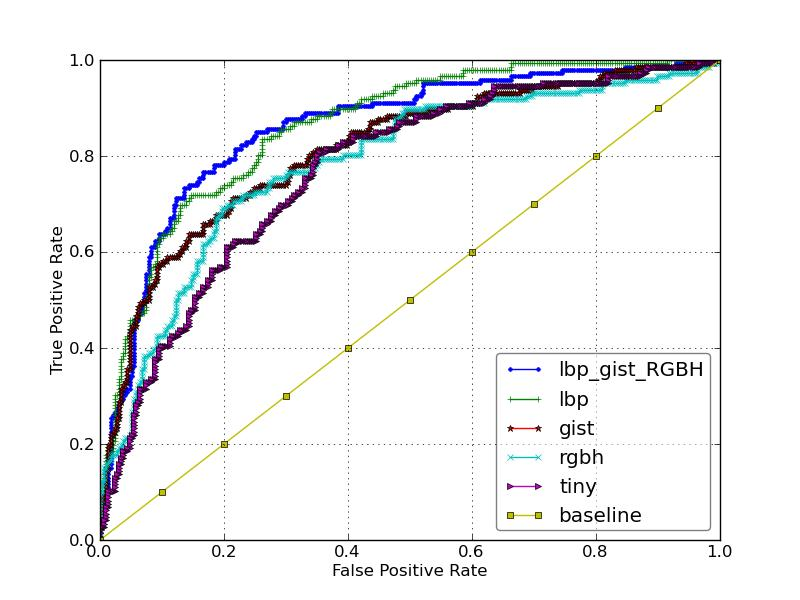
\includegraphics[width=0.4\textwidth]{figs/ROC-curves_poppytype1.jpg} &
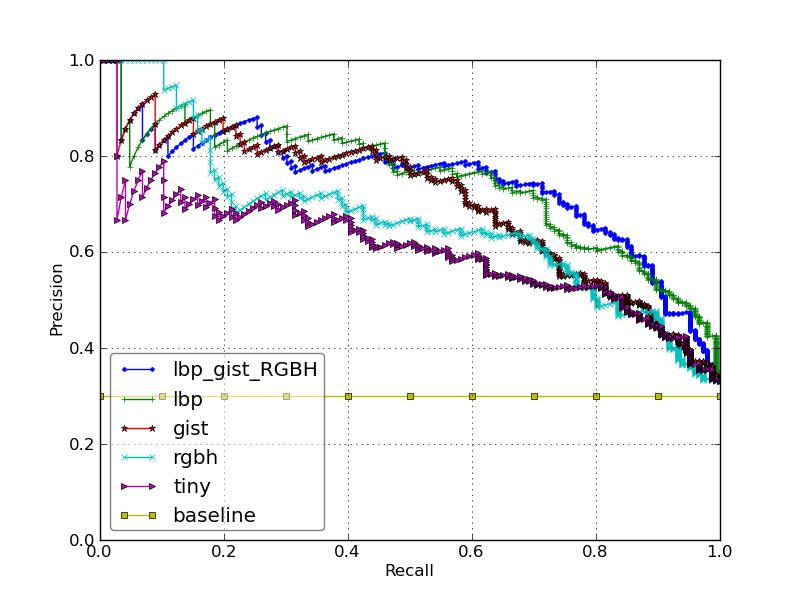
\includegraphics[width=0.4\textwidth]{figs/PR-curves_poppytype1.jpg} \\
\end{tabular}
\end{center}
\vspace{-12pt}
\caption{
California Poppy classification results for different features, where the goal is to find close-up pictures of California Poppies, in terms of {\textit{(left):}} ROC curves of classification performance and
{\textit{(right):}} Precision-Recall curves showing retrieval performance.
}
\label{fig:PR_ROC_poppy}
\end{figure*}




